\subsection{Arbres BSP en deux dimensions}
Les arbres BSP (binary space partition) sont la structure principale
intervenant dans l'algorithme du peintre. En deux dimensions, ils sont
utilisés pour stocker des ensembles de segments destinés à être affichés.


Soit
\begin{equation} \label{lin:forme}
f: \mathbb R^2 \to \mathbb R: (x, y)\mapsto a_1x +a_2y
\end{equation}
une forme linéaire, et $c\in\mathbb R$ un réel. Alors, il est possible de
partionner le plan $\mathbb R^2$ en trois sous-ensembles en le séparant
par la droite $D = \{v\in\mathbb R^n\mid f(v) = c\}$; les demi-plans
$D^+ = \{v\in\mathbb R^2\mid f(v) > c\}$,
$D^- = \{v\in\mathbb R^2\mid f(v) < c\}$ et la droite $D$ elle-même
(voir figure \ref{sep:ill}).

\begin{figure}[!h]
  \begin{center}
    \caption{Partition du plan par une droite et deux demi-plans}%
    \label{sep:ill}
    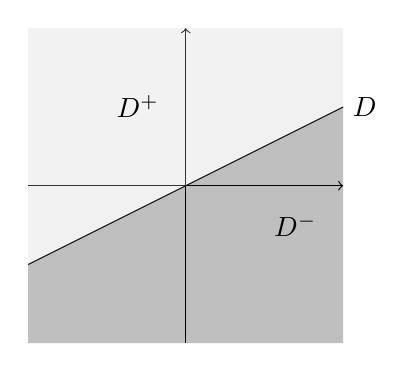
\begin{tikzpicture}
      \draw [->] (0, -2) -- (0, 2);
      \draw [->] (-2, 0) -- (2, 0);
      \draw (-2, -1) -- (2, 1) node[right] {$D$};
      \fill [black, nearly transparent] %
      (-2, -1) -- (2, 1) -- (2, -2) -- (-2, -2) -- cycle;
      \draw (1, -0.5) node[right] {$D^-$};
      \fill [black!20, nearly transparent] %
      (-2, -1) -- (2, 1) -- (2, 2) -- (-2, 2) -- cycle;
      \draw (-1, 1) node[right] {$D^+$};
    \end{tikzpicture}
\end{center}
\end{figure}

%%% Local Variables:
%%% mode: latex
%%% TeX-master: "../rapportGp1"
%%% End:


\begin{df}
  Un arbre BSP $T$ est un arbre binaire tel que:
  \begin{enumerate}
  \item Chaque noeud contient un ensemble $S$ de segments (éventuellement
    vide).
  \item Chaque noeud contient une équation de droite $D\equiv f(x, y) = c$ (où $f$
    est une forme linéaire et $c$ est un nombre réel).
  \item Tout segment dans $S$ est contenu dans la droite $D$.
  \item Chaque segment stocké dans le fils gauche $T^-$ (resp.
    le fils droit $T^+$) d'un noeud est contenu dans le demi-plan
    $D^-$ (resp. $D^+$).
  \end{enumerate}
\end{df}

Afin de construire des arbres BSP à partir d'une liste $L$ de segments
du plan, il faut à chaque fois sélectionner une droite par laquelle
séparer l'espace. Afin d'assurer que la construction de l'arbre BSP
est finie, la contrainte suivante est adoptée;
seules les droites comportant un segment de $L$ sont sélectionnées comme
droites séparatrices.
Le lemme suivant montre qu'il est possible d'obtenir une équation de droite
à partir d'un segment non dégénéré, en temps constant.

\begin{lem}\label{lem:droite}
  Soient $p_1 = (x_1, y_1)$ et $p_2 = (x_2, y_2)$ deux points distincts du
  plan. Une équation cartésienne de la droite  passant par $p_1$ et $p_2$
  est donnée par
  \begin{equation}
    \left(y_2 - y_1\right) x + \left(x_1 - x_2\right) y =
    \left(y_2 - y_1\right) x_1 + \left(x_1 - x_2\right) y_1
  \end{equation}
\end{lem}
\begin{proof}
  Le vecteur $(x_2 - x_1, y_2 - y_1)$ est un vecteur directeur de la droite.
  Alors $(y_2 - y_1, x_1 - x_2)$ est un vecteur normal de la droite ce qui
  implique que
  $\left(y_2 - y_1\right) x + \left(x_1 - x_2\right) y = c$ est une équation
  de la droite, où $c$ est à déterminer. Il suffit de poser
  $c = \left(y_2 - y_1\right) x_1 + \left(x_1 - x_2\right) y_1$
  car le point $(x_1, y_1)$ appartient à la droite.
\end{proof}

Le lemme \ref{lem:droite} fournit une équation d'une droite passant par
par deux points distincts en temps constant (il suffit d'effectuer
quelques opérations arithmétiques élémentaires). Le choix du segment
pour la partition est effectué selon une heuristique (se référer à la section
{\Huge \underline{\textsl{\textbf{REF}}}}).

Une fois la droite $D$ choisie, l'arbre est construit récursivement.
Deux nouvelles listes, $L_d$ et $L_g$ sont créées pour construire récursivement
les sous-arbres gauche et droit.

Si un segment $s$ de $L$ est compris dans la droite $D$, il est stocké à
la racine de l'arbre, dans l'ensemble $S$. Si un segment est contenu dans
le demi-plan $D^+$ (resp. $D^-$), il est stocké dans la liste $L_d$ (resp.
$L_g$). Si $s$ est à la fois dans $D^+$ et dans $D^-$ (c'est-à-dire une
extrémité est dans $D^+$ et l'autre dans $D^-$), il est nécessaire
de briser le segment en deux parties, qui seront ensuite ajoutés à une des
listes selon la dichotomie précédente.

Le résultat suivant fournit une solution en temps constant pour calculer
cette intersection, sous l'hypothèse qu'elle existe.

\begin{lem}
  Soit $D\equiv ax + by = c$ une droite du plan. Soient $p_1 = (x_1, y_1)$
  et $p_2 = (x_2, y_2)$ deux points tels que $p_1\in D^+$ et $p_2\in D^-$.

  Alors l'intersection du segment $[p_1, p_2]$ est donnée par $t_0p_1 + (1-t_0)p_2$
  où $t_0 = $.
\end{lem}
\begin{proof}
  Tout point de $[p_1, p_2]$ s'écrit $tp_1 + (1-t)p_2$ pour un certain
  $t\in [0, 1]$.
  L'intersection vérifie $f(t_0p_1 + (1-t_0)p_2) = c$. La linéarité de la
  fonction $f$ fournit $$t_0 = \frac{c-f(p_2)}{f(p_1)-f(p_2)}.$$
\end{proof}

Ces deux résultats permettent de donner l'algorithme de construction de
l'arbre (voir l'algorithme \ref{algo:bsp}).
\begin{algorithm}
  \caption{Build\_BSP($L, h$)}
  \begin{algorithmic}[1] \label{algo:bsp}
    \REQUIRE Une liste de segments $L$ et $h$ une fonction
    heuristique de sélection de segment (prenant une liste en paramètre).
    \ENSURE -- (construit un arbre BSP représentant l'ensemble de segments $L$)
    \IF{$L$ est vide}
    \STATE $T\leftarrow$ Feuille()
    \ENDIF
    \IF{$L$ est non vide}
    \STATE $L_g\leftarrow$ Liste()
    \STATE $L_d\leftarrow$ Liste()
    \STATE $S \leftarrow \varnothing$
    \STATE $f\leftarrow$ équation de la droite passant par le segment $h(L)$
    \FOR{$s=[p_1, p_2]\in L$} \label{bsp:for}
    \IF{$f(p_1) = c$ et $f(p_2) = c$}
    \STATE $S\leftarrow S\cup\{s\}$
    \ELSIF{$f(p_1)\geq c$ et $f(p_2)\geq c$}
    \STATE Ajouter $s$ à $L_d$
    \ELSIF{$f(p_1)\leq c$ et $f(p_2)\leq c$}
    \STATE Ajouter $s$ à $L_g$
    \ELSE
    \STATE $p_3\leftarrow [p_1, p_2]\cap D$
    \COMMENT{Les cas sans intersections sont épuisés}
    \IF{$f(p_1)>c$ et $f(p_2) < c$}
    \STATE Ajouter $[p_1, p_3]$ à $L_d$
    \STATE Ajouter $[p_3, p_2]$ à $L_g$
    \ELSE
    \STATE Ajouter $[p_1, p_3]$ à $L_g$
    \STATE Ajouter $[p_3, p_2]$ à $L_d$
    \ENDIF
    \ENDIF
    \ENDFOR
    \STATE $T^+\leftarrow$Build\_BSP($L_d$, $h$)
    \STATE $T^-\leftarrow$Build\_BSP($L_g$, $h$)
    \ENDIF
  \end{algorithmic}
\end{algorithm}

\begin{prop}
  L'algorithme de construction d'arbre BSP se termine.
\end{prop}
\begin{proof}
  Prouvons ceci par induction sur la taille de la liste.
  Si la liste est vide (cas de base), alors l'algorithme n'effectue
  pas d'appel récursif et s'arrête.

  Soit $n\geq 1$ un naturel. Supposons désormais (par induction) que pour
  tout naturel $k\in\{0, \ldots, n-1\}$, l'algorithme s'arrête pour
  une entrée de taille $k$. Montrons que si une liste de taille $n$
  est donnée en entrée, alors l'algorithme s'arrête.

  Il suffit de montrer que les listes $L_g$ et $L_d$ sont de taille
  au plus $n-1$. \`{A} chaque passage dans la boucle pour (ligne \ref{bsp:for}), un segment
  est placé soit dans l'ensemble $S$, soit dans une des deux listes
  $L_g$ ou $L_d$, ou bien il est éclaté en deux moitiés placées
  dans une liste chacune. En particulier, au cours d'une itération,
  la taille des listes n'augmente pas si un segment est placé dans $S$
  et sinon augmente d'au plus d'une unité.

  Par choix de la droite de séparation,
  au moins un segment y est inclus; dès lors, ce segment est stocké
  dans $S$. Ceci implique que $L_d$ et $L_g$ contiennent au plus $n-1$
  éléments, ce qui assure l'arrêt de l'algorithme par hypothèse d'induction.
\end{proof}


\section{Algorithme du peintre}
L'algorithme du peintre est un algorithme permettant d'effectuer un
affichage sans afficher les objets cachés par d'autres (\emph{hidden surface
  removal}). \`{A} la manière d'un peintre, le principe de l'algorithme est
de dessiner les objets dans un ordre tel qu'aucun objet à l'arrière-plan
(vis-à-vis du point de vue) n'obscurcisse d'objet à l'avant-plan.
\section{Calcul des parties visibles}



%%% Local Variables:
%%% mode: latex
%%% TeX-master: "../rapportGp1"
%%% End:
